\documentclass[a4paper,11pt,notitlepage]{report}

\usepackage{graphicx}
\usepackage[utf8]{inputenc}
\usepackage[T1]{fontenc}
\usepackage[ngerman]{babel}
\usepackage{bibgerm}
\usepackage{amsmath,amssymb,amsthm}
\usepackage{color}
\usepackage{enumerate}
\usepackage{tabularx}
\usepackage{subfig}
\usepackage{fancyhdr}
\usepackage{upgreek}
\usepackage[pdftex,pdfpagelabels,colorlinks,backref,pagebackref]{hyperref}
\usepackage{tikz} % SELBST HINZUGEFÜGT
\usepackage{graphicx}
% == Set the heading style ===================================================
\setlength{\headheight}{14pt}
\pagestyle{fancyplain}
\renewcommand{\chaptermark}[1]{\markboth{#1}{}}
\renewcommand{\sectionmark}[1]{\markright{\thesection\ #1}}
\lhead[\fancyplain{}{\thepage}]{\fancyplain{}{\rightmark}}
\rhead[\fancyplain{}{\leftmark}]{\fancyplain{}{\thepage}}
\cfoot{}
\renewcommand{\headrulewidth}{0.4pt}
% ============================================================================

% == Set correct values for fitting floats ===================================
\tolerance=2000
\emergencystretch=10pt

\setcounter{topnumber}{3}
\setcounter{totalnumber}{5}
\setcounter{bottomnumber}{2}

% To make those darn floats fit where they should
\setcounter{totalnumber}{9}
\setcounter{topnumber}{9}
\setcounter{bottomnumber}{9}
\renewcommand{\textfraction}{0.00}
\renewcommand{\topfraction}{1.0}
\renewcommand{\bottomfraction}{1.0}
% ============================================================================

% == German definitions for theorems etc. ==================================== 
\newtheorem{definition}{Definition}[chapter]
\newtheorem{theorem}{Satz}[chapter]
\newtheorem{lemma}{Lemma}[chapter]
\newtheorem{proposition}{Proposition}[chapter]
\newtheorem{corollary}{Korollar}[chapter]
\newtheorem{observation}{Beobachtung}[chapter]
\newtheorem{fact}{Fakt}[chapter]
\newtheorem{remark}{Bemerkung}[chapter]
\newtheorem{example}{Beispiel}[chapter]
% ============================================================================

% == Abkürzungen für die reellen, natürlichen, ganzen,... Zahlen =============
\newcommand{\R}{{\ensuremath{\mathbb{R}}}}
\newcommand{\N}{{\ensuremath{\mathbb{N}}}}
\newcommand{\Z}{{\ensuremath{\mathbb{Z}}}}
\newcommand{\C}{{\ensuremath{\mathbb{C}}}}
\newcommand{\Q}{{\ensuremath{\mathbb{Q}}}}
\newcommand{\F}{{\ensuremath{\mathbb{F}}}}
\newcommand{\Prim}{{\ensuremath{\mathbb{P}}}}
% ============================================================================

% == Makros für Autorenname und -adresse =====================================
\newcommand{\myaddress}[6]{%
  \parbox{\textwidth}{\textbf{\large #1}\\
    #2\\ #3\\ #4\\ 
    \ifthenelse{\equal{#5}{}}{}{Email: \href{mailto:#5}{\texttt{#5}}\\}
    \ifthenelse{\equal{#6}{}}{}{WWW: \href{#6}{\path|#6|}\\}
  } 
}

\newcommand{\myauthor}[1]{%
  \addtocontents{toc}{\protect\hspace{3.35ex}%
  \textsl{#1}\par}\vspace{-4ex}\quad\hfill\textsl{\Large #1}\vspace{8ex}}

\newcommand{\myname}[1]{\Large #1}

%%%%%%%%%%%%%%%%%%%%%%%%%%%%%%%%%%%%%%%%%%%%%%%%%%
% Tragen Sie in der folg. Zeile Ihren Namen ein: %
%%%%%%%%%%%%%%%%%%%%%%%%%%%%%%%%%%%%%%%%%%%%%%%%%%

\newcommand{\OO}{{\ensuremath{\upsigma}}}

\begin{document}
\shorthandoff{"}

\begin{titlepage}
	\begin{center}	
		\LARGE \textbf{{Einführung in die Geometrie und Topologie - Mitschrieb -} \\[5ex] 
    		{\Large Vorlesung im Wintersemester 2011/2012\\[5ex]}}
	\end{center}
	\begin{center}
		\Large Sarah Lutteropp
	\end{center}
	\begin{center}
		\today
	\end{center}
	\vspace{2cm}
	\begin{center}
		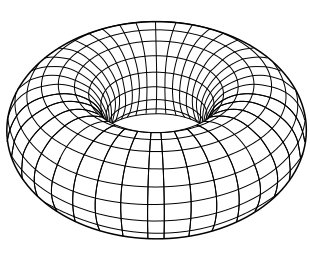
\includegraphics[width=0.8\textwidth]{Simple_Torus.jpg}
	\end{center}
\end{titlepage}
%\maketitle
\setcounter{tocdepth}{1}
\tableofcontents

\section*{Vorwort}
Dies ist ein Mitschrieb der Vorlesung “Einführung in die Geometrie und Topologie” vom Wintersemester 2011/2012 am Karlsruher Institut für Technologie, die von Herrn Prof. Dr. Wilderich Tuschmann gehalten wird.

\chapter{Homotopie und Fundamentalgruppe}

\begin{definition}[Topologischer Raum]
Ein \underline{topologischer Raum} $X$ ist gegeben durch eine Menge $X$ und ein System $\OO$ von Teilmengen von $X$, den so genannten \underline{offenen Mengen} von $X$, welches unter beliebigen Vereinigungen und endlichen Durchschnitten abgeschlossen ist und $X$ und die leere Menge $\emptyset$ als Elemente enthält.
\newline
$X$ Menge, $\OO \subset \mathcal{P}(X) \colon$
\begin{itemize}
	\item (1) $O_1, O_2 \in \OO \Rightarrow O_1 \cap O_2 \in \OO$
	\item (2) $O_\alpha \in \OO, \alpha \in A, A \text{ Indexmenge} \Rightarrow \bigcup\limits_{\alpha \in A}{O_\alpha} \in \OO$
	\item (3) $X, \emptyset \in \OO$
\end{itemize}
\end{definition}

\begin{example}
\OO = $\{X, \emptyset\} \Rightarrow (X,\OO)$ ist topologischer Raum!
\end{example}

\begin{example}
$$X \text{ Menge, }\OO = \left\{\{x\}|x\in X\right\} + \text{Axiome, die zu erfüllen sind} \leadsto \tilde{\OO}$$
$\Rightarrow (X,\tilde{\OO})$ ist topologischer Raum.
$\OO$ ist "Basis" der Topologie $\tilde{\OO}$.
\end{example}

\begin{definition}[Metrischer Raum]
Ein \underline{metrischer Raum} $X$ ist eine Menge $X$ mit einer Abbildung $d \colon X \times X \rightarrow \R$, der \underline{"Metrik"} auf $X$, die folgende Eigenschaften erfüllt:

\begin{itemize}
	\item (1) $d(x,y) = d(y,x)$ \underline{"Symmetrie"}
	\item (2) $d(x,y) = 0 \Leftrightarrow x = y, d(x,y) \geq 0$ \underline{"Definitheit"}
	\item (3) $d(x,z) \leq d(x,y) + d(y,z)$ \underline{"Dreiecksungleichung"}
	\item $\forall x,y,x \in X$
\end{itemize}

\end{definition}

\begin{definition}[stetig]
Eine Abbildung $F \colon X \rightarrow Y$ zwischen topologischen Räumen $X$ und $Y$ heißt \underline{stetig}, falls die F-Urbilder offener Mengen in $Y$ offene Teilmengen von $X$ sind.
\end{definition}

\begin{remark}
Ist $(X,d)$ ein metrischer Raum, so sind die offenen Mengen der von der Metrik induzierten Topologie Vereinigungen von endlichen Durchschnitten von Umgebungen
$U_{\epsilon}(x):=\{y \in X | d (x,y) < \epsilon \} (\epsilon > 0)$, 
und $F \colon (X,d) \rightarrow (Y,d')$ ist stetig im obigen Sinn genau dann, falls für alle $\epsilon > 0$ ein $\delta > 0$ existiert mit $F(U_\delta (x)) \subset U_\epsilon (F(x))$.
\end{remark}

\begin{definition}[Homotopie]
Eine \underline{Homotopie} $H \colon f \simeq g$ zwischen zwei (stetigen) Abbildungen $f,g \colon X \rightarrow Y$ ist eine (stetige) Abbildung $$H \colon X \times I \footnote{$I = [0,1] \subset \R$} \rightarrow Y, (x,t) \mapsto H(x,t)$$ mit $H(x,0) = f(x) \text{ und } H(x,1) = g(x) \forall x \in X$.
\end{definition}

TODO:BILDER

\begin{remark}
$H$ heißt auch \underline{Homotopie} \underline{\underline{von $f$ nach $g$}}, eine solche ist also eine parametrisierte Schar von Abbildungen mit "Anfang" $f$ und "Ende" $g$. $f$ und $g$ heißen dann \underline{homotop}, in Zeichen: $f \simeq g$.
\end{remark}

\paragraph{Erinnerung}
Sind $X$ und $Y$ topologische Räume, so ist eine Homotopie $H = (h_t), t \in [0,1]$, eine parametrisierte Schar von stetigen Abbildungen $h_t \colon X \rightarrow Y$ mit \underline{Anfang} $h_0$ und Ende $h_1$. (TODO: BILD)

\begin{definition}[homotope Abbildungen]
	Zwei (stetige) Abbildungen heißen \underline{homotop}, in Zeichen: $f \simeq g$, falls eine Homotopie mit Anfang $f$ und Ende $g$ existiert.
\end{definition}

\begin{remark}
"Homotop sein" ist eine Äquivalenzrelation.
\end{remark}

\begin{proof}
	\underline{Symmetrie}:
	Gilt für $f,g \in C(X,Y) := \{F \colon X \rightarrow Y \text{ stetig } \}$ $f \simeq g$ vermöge $H=(h_t), t \in [0,1],$ so liefert $(\tilde{h_t}) mit \tilde{h_t}:=h_{1-t}$ eine Homotopie von $g$ nach $f$, d.h. $f \simeq g \Leftrightarrow g \simeq f$.
	\newline
	\underline{Reflexivität}:
	$f \simeq f$ vermöge $h_t : \equiv f \forall t \in [0,1]$
	\newline
	\underline{Transitivität}:
	Es sei $f \simeq g$ vermöge $(h_t)$ und ferner $g \simeq l$ vermöge $(k_t)$.
	Dann liefert $M \colon X \times [0,1] \rightarrow Y$ mit
	$$M_t := \begin{cases} h_{2t} & 0 \leq t \leq \frac{1}{2} \\
	k_{2t-1} & \frac{1}{2} \leq t \leq 1
	\end{cases}$$
	eine Homotopie von $f$ nach $l$.
	\newline
	Also ist $f \simeq g, g \simeq l \Rightarrow f \simeq l$.
\end{proof}
(TODO:BILD)

\begin{remark}
Die Äquivalenzrelation "Homotopie von Abbildungen" liefert also eine Partition von $C(X,Y)$ in Äquivalenzklassen. Diese heißen Homotopieklassen und die \underline{Menge aller Homotopieklassen stetiger Abbildungen von $X$ nach $Y$} wird mit $[X,Y]$ bezeichnet.
(TODO: BILD)
\end{remark}

\begin{remark}
$C(X,Y)$ ist im Allgemeinen \underline{\underline{viel}} schwieriger zu verstehen als $[X,Y]$!
\end{remark}

\begin{example}
Je zwei stetige Abbildungen $f,g \colon X \rightarrow \R^n$ sind homotop! Denn $H(x,t):= (1-t) f(x) + t \cdot g(x)$ liefert eine Homotopie von $f$ nach $g$: (TODO: BILD)
\end{example}

\begin{definition}
Eine stetige Abbildung $f \colon X \rightarrow Y$ heißt \underline{nullhomotop}, falls sie homotop zu einer konstanten Abbildung ist. (TODO:BILD)
\end{definition}

\begin{corollary}
Jede stetige Abbildung $f \colon X \rightarrow \R^n$ ist nullhomotop, d.h. für jeden topologischen Raum $X$ besteht $[X, \R^n]$, $n$ beliebig, nur aus einem Punkt!
\end{corollary}

\begin{example}
Jeder \underline{geschlossene Weg im $\R^2$}, d.h. jede stetige Abbildung $f \colon [0,1] \rightarrow \R^2$ mit $f(0) = f(1)$ ist nullhomotop.
$\bigl[[0,1], \R^2\bigr]$ + gleicher Anfangs- und Endpunkt besteht nur aus einem Punkt, zum Beispiel der Äquivalenzklasse der konstanten Kurve $t \mapsto (1,0)$. (TODO: BILD)
Interpretiere einen geschlossenen Weg im $\R^2$ auch als stetige Abbildung von $S^1$ in $\R^2$, so gilt also $[S^1, \R^2]$ ist einelementig.
\newline
\underline{Aber} $[S^1, \R^2 \backslash \{0\}]$ ist nichttrivial! (TODO: BILD)
\end{example}

\begin{definition}
Es sei $(X, \OO)$ topologischer Raum und $A \subset X$. Die auf $A$ durch
$$\OO \Big |_{A} := \{U \cap A | U \in \OO \}$$
induzierte Topologie heißt \underline{Teilraumtopologie} und der dadurch gegebene topologische Raum $(A, \OO \Big |_{A})$ heißt \underline{Teilraum} von $(X, \OO)$.
\end{definition}

\begin{remark}
$B \subset A$ ist also genau dann \underline{offen \underline{in $A$}}, wenn $B$ der Schnitt einer \underline{in $X$} offenen Menge mit $A$ ist.
\end{remark}

\begin{example}
$X = \R^2, A = S^1 = \{ x \in \R^2 |\text{ } ||x|| = 1\}$ 
\newline
(TODO: BILD)
\newline
\underline{Achtung:} $B$ ist \underline{\underline{nicht}} offen in $R^2$!
\end{example}

\chapter{Grundlagen der allgemeinen Topologie}
\begin{example}[Beispiele topologischer Räume]
	\begin{itemize}
		\item (1) $X, \OO := \{X, \emptyset\}$ \underline{`triviale Topologie'}
		\item (2) $X, \OO := \mathcal{P}(X)$ \underline{`diskrete Topologie'}
		\item (3) Metrische Räume, siehe unten
		\item (4) $X:= \{a,b,c,d\} \Rightarrow \OO := \left\{X, \emptyset, \{a\}, \{b\}, \{a,c\}, \{a,b,c\}, \{a,b\} \right \}$ definiert eine Topologie auf $X$, aber $\OO^\prime:= \left \{ X, \emptyset, \{a,c,d\}, \{b,d\} \right \}$ nicht!
		\item (5) $X := \R, \OO := \{O \mid \text{O ist Vereinigung von Intervallen } (a,b) \text{ mit } a,b \in \R\}$. $\Rightarrow (X, \OO) \text{ ist topologischer Raum}$, und $\OO$ heißt \underline{Standard-Topologie}.
		\item (6) $X:= \R, \tilde{\OO} := \{O \mid O = \R \backslash E, E \subset \R \text{ endlich}\} \cup \{\emptyset\}$ ist auch eine Topologie auf $\R$, die so genannte $\tau_1$-Topologie.
	\end{itemize}
\end{example}

\begin{definition}
	$A \subset X, X$ topologischer Raum, heißt \underline{abgeschlossen} $:\Leftrightarrow X \backslash A \text{ ist offen}$.
\end{definition}

\begin{remark}
	Beliebige Durchschnitte abgeschlossener Mengen sind abgeschlossen, ebenso endliche Vereinigungen und genauso $X$ und $\emptyset$.
\end{remark}

\begin{example}
	In einem diskreten topologischen Raum sind \underline{alle Teilmengen} abgeschlossen, in $\R_{\tau_1}$\footnote{$\R$ mit $\tau_1$-Topologie} alle endlichen Teilmengen und $X, \emptyset$.
\end{example}

\begin{definition}
	Ist $X$ topologischer Raum und $x \in X$, so heißt jede \underline{offene} Teilmenge $O \subset X$ mit $x \in O$ eine \underline{Umgebung} von $x$.
\end{definition}

\begin{remark}
	Umgebungen sind per definitionem offen! (TODO: BILD)
\end{remark}

\begin{remark}
	Jede offene Teilmenge von $\R_{Standard}$ ist eine Vereinigung disjunkter offener Intervalle, doch abgeschlossene Teilmengen von $\R$ sind keinesfalls immer Vereinigungen abgeschlossener Intervalle!
\end{remark}

\begin{example}[Die \underline{Cantor-Menge} $\mathcal{C}:= \left \{ x \in \R \mid x = \sum\limits_{k=1}^{\infty}{\frac{a_k}{3^k}}, a_k \in \{0,2\} \right \}$]
	(TODO: BILD)
	\newline
	$\Rightarrow$ $\mathcal{C}$ ist abgeschlossen in $\R$, enthält überabzählbar viele Elemente und hat `Hausdorff-Dimension' $\frac{\ln 2}{\ln 3} \approx 0,6 \ldots$
\end{example}

\begin{definition}
	Ist $(X, \OO)$ topologischer Raum mit $\mathcal{B} \subset \OO$, so heißt $\mathcal{B}$ \underline{Basis der Topologie} $:\Leftrightarrow$ Jede (nichtleere) offene Menge ist Vereinigung von Mengen aus $\mathcal{B}$.
\end{definition}

\begin{example}
	$\bullet$ (1) Die offenen Intervalle bilden eine Basis der Standard-Topologie von $\R$.
	\newline
	$\bullet$ (2) Sämtliche offenen\footnote{bezüglich der euklidischen Metrik} Kreisscheiben (TODO: BILD) und auch sämtliche offenen Quadrate (TODO: BILD) bilden Basen ein und derselben Topologie auf $\R^2$.
	\newline
	(TOSO: BILD)
\end{example}

\begin{remark}
	$\bullet$ $\mathcal{B} \subset \OO$ ist Basis der Topologie von $X$ $\Leftrightarrow \forall O \in \OO \forall x \in O \exists B \in \mathcal{B} \colon x \in B \subset O$.
	\newline
	$\bullet$ $\mathcal{B} \subset \mathcal{P}(X)$ bildet die Bais \underline{einer} Topologie auf $X$ $\Leftrightarrow$ $X$ ist Vereinigung von Mengen aus $\mathcal{B}$ und der Schnitt je zweier Mengen aus $\mathcal{B}$ ist eine Bereinigung von Mengen aus $\mathcal{B}$.
	\newline
	(TODO: BILD)
\end{remark}

\begin{definition}
	Seind $\OO_1$ und $\OO_2$ Topologien auf $X$ und $\OO_1 \subset \OO_2$, so heißt $\OO_2$ \underline{feiner} als $\OO_1$ und $\OO_1$ \underline{gröber} als $\OO_2$.
\end{definition}

\begin{example}
	$\bullet$ Die triviale Topologie ist die gröbste Topologie auf $X$, die diskrete Topologie die feinste.
	\newline
	$\bullet$ Die Standard-Topologie auf $\R$ ist feiner als die $\tau_1$-Topologie.
\end{example}

\paragraph{Mehr in metrischen Räumen:}

\begin{definition}
	Für einen metrischen Raum $(X,d)$ und $\epsilon > 0$ sei für $p \in X$
	\begin{itemize}
		\item $B_\epsilon(p):=\{x \in C \mid d(p,x) < \epsilon \}$ der \underline{offene $\epsilon$-Ball um $p$}
		\item $D_\epsilon(p):=\{x \in C \mid d(p,x) \leq \epsilon \}$ der \underline{abgeschlossene $\epsilon$-Ball um $p$}
		\item $S_\epsilon(p):=\{x \in C \mid d(p,x) = \epsilon \}$ die \underline{ $\epsilon$-Sphäre} um $p$ (oder \underline{Sphäre vom Radius $\epsilon$})
	\end{itemize}
\end{definition}

\begin{definition}
	Ist $(X,d)$ metrischer Raum und $A \subset X$, so heißt der metrische Raum $(A, d \big |_{A \times A})$ \underline{(metrischer) Unterraum von $X$}.
\end{definition}

\begin{example}
	Für $X=\R_{Eukl.}^{n}$ sind $B_1(0), D_1(0) =: D^n$ und $S^{n-1}:=S_1{0}$ metrische Unterräume und heißen auch offener bzw. abgeschlossener Einheitsball bzw. $(n-1)$-Sphäre.
	\newline
	(TODO: BILD)
\end{example}

\begin{definition}
	$A \subset (X,d)$ heißt \underline{beschränkt} \newline $:\Leftrightarrow \exists 0 < \rho \in \R \colon d(x,y) < \rho  \text{   } \forall x,y \in A$
	\newline
	(TODO: BILD)
	\newline
	Das Infimum, diam $A$, dieser $\rho$ heißt dann \underline{Durchmesser von $A$}.
\end{definition}

\begin{remark}
	In einem metrischen Raum $(X,d)$ bilden die offenen Bälle die Basis einer Topologie $\OO=\OO_d$ von $X$, diese heißt \underline{die von der Metrik induzierte Topologie}.
\end{remark}

\begin{remark}
	$A \subset (X,d)$ ist dann \underline{offen} $\Leftrightarrow \forall p \in A \exists \text{ ein offener Ball } B_\epsilon(p) \text{ um } p \text{ mit } B_\epsilon(p) \subset A$
	\newline
	(TODO: BILD)
\end{remark}

\begin{definition}
	$(X,d)$ sei metrischer Raum und $A \subset X, p \in X$.
	$$d(p,A) := dist(p,A):= \inf \{d(p,a) \mid a\in A \}$$
	heißt \underline{Abstand von $p$ und $A$}.
\end{definition}

\end{document}
